\chapter{Newtonsche Kosmologie und die Friedmann-Gleichung}

Letztes Mal haben wir über die Metrik des Raums gesprochen. Als Nächstes geht es um die Dynamik: Wie ändert sich der Skalenfaktor mit der Zeit? Zunächst betrachten wir ein wenig Geometrie und anschließend die Newtonsche Kosmologie. Die Friedmann-Gleichung wird hier noch nicht aus der allgemeinen Relativitätstheorie hergeleitet, sondern aus den Newtonschen Gleichungen.

\section{Homogenität, Isotropie und eine zeitabhängige Metrik}

Homogenität und Isotropie sind die grundlegenden Annahmen. Ist das Universum homogen und isotrop und verändert es sich mit der Zeit, dann gilt das Hubble-Gesetz stets. Zu jedem festgelegten Zeitpunkt ist die Fluchtgeschwindigkeit proportional zur Entfernung,
\begin{equation}
v = H(t)\,d.
\end{equation}
und zwar linear. Nicht die Zeit, sondern der Raum ist hier maßgeblich: Zu einem gegebenen Zeitpunkt gilt überall derselbe Proportionalitätsfaktor.

\begin{classroomqa}
\audiencequestion{Heißt das, dass die Proportionalität linear ist?}\lecturetimestamp{00:02:06}
\lecturerresponse{Ja. Zu einem festen Zeitpunkt ist die Fluchtgeschwindigkeit linear proportional zur Entfernung. Der Proportionalitätsfaktor ist die Hubble-Konstante. Im Allgemeinen hängt sie von der Zeit ab, variiert aber nicht von Ort zu Ort im Raum.}
\end{classroomqa}

Deshalb ist die Bezeichnung ``Hubble-Konstante'' irreführend. Sie ist bezüglich des Ortes im Raum konstant, nicht aber bezüglich der Zeit.

Eine naheliegende Frage lautet nun: Wenn sich der Raum ausdehnt, warum dehnen sich dann Meterstäbe nicht ebenfalls aus? Die Antwort lautet, dass Meterstäbe durch Kräfte zusammengehalten werden, die sehr viel stärker sind als alles, was mit der kosmologischen Expansion auf atomaren Skalen zusammenhängt. Gebundene Objekte bleiben gebunden. Was sich ausdehnt, ist der Abstand zwischen hinreichend voneinander getrennten Dingen, etwa zwischen Galaxien, die so weit auseinanderliegen, dass sie einander nicht stark zusammenhalten.

\begin{classroomqa}
\audiencequestion{Gibt es ein Problem damit, dass sich die Messstäbe ebenfalls ausdehnen?}\lecturetimestamp{00:04:00}
\lecturerresponse{Nein. Die Messstäbe dehnen sich nicht aus. Die Koordinaten dehnen sich aus. Die Kräfte, die Meterstäbe zusammenhalten, sind viel stärker als die Auswirkungen der Expansion. Daher dehnen sich gewöhnliche gebundene Objekte nicht mit dem Hintergrund aus. Galaxien, die weit genug voneinander entfernt sind, entfernen sich voneinander, Meterstäbe jedoch nicht.}
\end{classroomqa}

Man kann sich sogar einen winzigen zusätzlichen abstoßenden Effekt zwischen Atomen vorstellen. Auch der würde einen Stab nicht auseinanderreißen. Er würde lediglich den Gleichgewichtsabstand ein wenig verschieben, so wie eine kleine zusätzliche Kraft die Gleichgewichtslage einer steifen Feder verändert.

\begin{classroomqa}
\audiencequestion{Man kann es aber nicht als Kraft zwischen Punkten modellieren, stimmt das? Denn sonst wäre es eine Beschleunigung.}\lecturetimestamp{00:05:29}
\lecturerresponse{Eine kleine zusätzliche Kraft zwischen Atomen kann man sich vorstellen. Ist sie jedoch winzig im Vergleich zu den Bindungskräften, verschiebt sie nur geringfügig die Gleichgewichtslage. Die Expansion allein erzeugt kein gewöhnliches Kraftgesetz. Manche Arten der Expansion lassen sich durch eine Kraft modellieren, nämlich die beschleunigte Expansion; das ist aber eine Frage für später.}
\end{classroomqa}

Nützlich sind also Koordinaten, die in die expandierende Materieverteilung eingebettet sind. Galaxien ohne zusätzliche Pekuliarbewegung behalten dieselben Koordinatenwerte. Was sich mit der Zeit ändert, ist die Beziehung zwischen dem Koordinatenabstand und dem in Metern gemessenen physikalischen Abstand. Diese Beziehung wird durch den Skalenfaktor \(a(t)\) beschrieben.

Für einen flachen Raum lässt sich die räumliche Metrik schreiben als
\begin{equation}
ds^2 = a(t)^2\left(dx^2+dy^2+dz^2\right).
\end{equation}
Hier ist \(a\) der tatsächliche, in Metern gemessene Abstand zwischen benachbarten Punkten, die im Koordinatenraum eine Einheit voneinander entfernt sind. Dehnt sich das Universum aus, wird \(a\) zeitabhängig.

Um zur Raumzeit überzugehen, geht man von der speziell-relativistischen Form
\begin{equation}
d\tau^2 = dt^2 - ds^2,
\end{equation}
aus und setzt die räumliche Metrik ein. Das ergibt
\begin{equation}
d\tau^2 = dt^2 - a(t)^2\left(dx^2+dy^2+dz^2\right).
\end{equation}
Die Koeffizienten hängen nicht vom Ort im Raum ab, sondern nur von der Zeit. In der Sprache der Metrik ist das die Aussage der Homogenität. Die Diagonalmetrik hat die Form
\begin{equation}
g_{\mu\nu}=\mathrm{diag}\!\left(1,-a(t)^2,-a(t)^2,-a(t)^2\right).
\end{equation}
\editorialnote{Die hier angegebene vollständige Diagonalmatrix entspricht der mündlichen Beschreibung des Metriktensors um 00:14:33. Der Tafelrahmen zeigt das Linienelement deutlich, aber keine vollständig lesbare Matrix.}

Es gibt keine Nebendiagonaleinträge: weder \(dx\,dy\) noch \(dx\,dt\) noch andere gemischte Terme. Die Metrik ist fast so einfach wie die der flachen Raumzeit. Das Besondere ist, dass die Beziehung zwischen räumlichem Maß und Zeit selbst zeitabhängig ist.

\begin{figure}
\centering
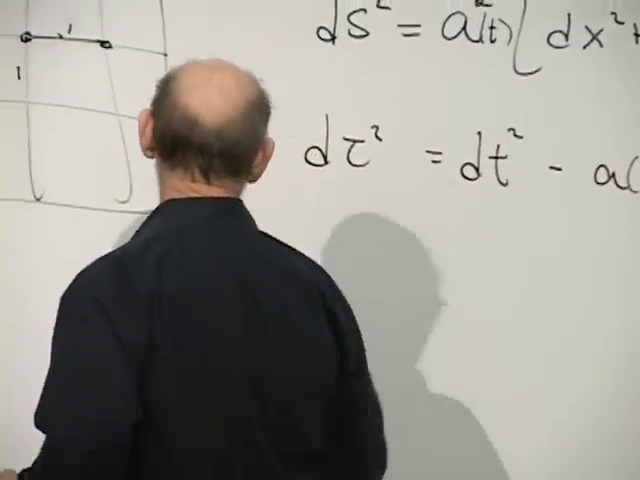
\includegraphics[width=0.62\textwidth]{lecture_02_figure_02.png}
\caption{Skizze eines mitbewegten Koordinatengitters und Raumzeitintervall mit zeitabhängigem Skalenfaktor.}
\end{figure}

Die Skizze verdeutlicht den entscheidenden Punkt. Alice und Bob bleiben in den mitbewegten Koordinaten eine Einheit voneinander entfernt, doch diese Koordinateneinheit entspricht mit der Zeit immer mehr Metern. Wäre \(a(t)\) zu einem Zeitpunkt in der Vergangenheit null gewesen, dann wären alle physikalischen Abstände null. Alles wäre zu einem einzigen Punkt zusammengedrängt. Deshalb entspricht \(a\to 0\) unendlicher Dichte. Wenn \(a\) wächst, wird das Universum immer diffuser.

Diese Form der Metrik gilt nicht in jedem Bezugssystem. Sie ist die Form im mit den Galaxien mitbewegten Bezugssystem.

\begin{classroomqa}
\audiencequestion{In dieser Gleichung: Die kleine Größe \(t\), \(a(t)\), wessen \(t\) ist das?}\lecturetimestamp{00:19:19}
\lecturerresponse{Das ist die Zeit, die von Uhren gemessen wird, die sich mit den Galaxien bewegen. Man stelle sich identische Uhren vor, die in derselben kosmischen Uhrenfabrik hergestellt und von den Galaxien mitgeführt werden. In diesem Bezugssystem entspricht die Zeitvariable genau dem, was diese Uhren messen. Entlang einer Galaxienweltlinie ist die Eigenzeit gleich dieser Koordinatenzeit.}
\end{classroomqa}

Tatsächlich gilt entlang der Weltlinie einer mitbewegten Galaxie
\begin{equation}
dx=dy=dz=0,
\end{equation}
also
\begin{equation}
d\tau^2 = dt^2,
\end{equation}
und damit
\begin{equation}
dt=d\tau.
\end{equation}

\begin{classroomqa}
\audiencequestion{Gibt es Transformationen, unter denen diese Form der Metrik invariant bleibt?}\lecturetimestamp{00:23:08}
\lecturerresponse{Ja, Rotationen, denn \(dx^2+dy^2+dz^2\) ist unter Rotationen invariant. Lorentz-Boosts erhalten diese Form dagegen nicht. Die Materie selbst zeichnet das mit den Galaxien mitbewegte Bezugssystem aus; in einem anderen Bezugssystem würde die Welt nicht isotrop erscheinen.}
\end{classroomqa}

\section{Ein Projektil in einem Gravitationsfeld}

Bevor wir die Newtonsche Mechanik auf das gesamte Universum anwenden, betrachten wir zunächst ein einfacheres Problem: eine große Masse \(M\), eine viel kleinere Masse \(m\) und einen anfänglichen Impuls nach außen. Nach diesem Impuls bewegt sich die kleine Masse einfach im Gravitationsfeld und verhält sich so, wie es Newtons Gesetze vorgeben.

Für die kosmologische Diskussion ist nicht das vollständige Bahnproblem entscheidend, sondern die Energieerhaltung. Die kinetische Energie lautet
\begin{equation}
\frac{1}{2}mv^2.
\end{equation}

\begin{figure}
\centering
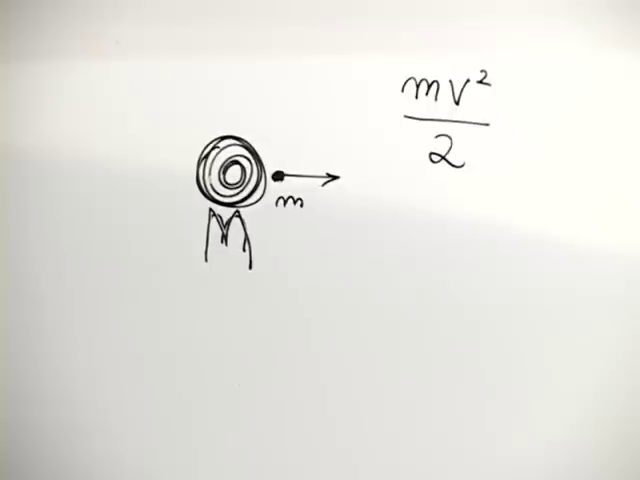
\includegraphics[width=0.42\textwidth]{lecture_02_figure_03.png}
\caption{Nach außen bewegte Testmasse und der Term für die kinetische Energie \(\frac{1}{2}mv^2\).}
\end{figure}

Die potenzielle Energie im Gravitationsfeld enthält das Produkt der Massen und der Newtonschen Gravitationskonstante; im Nenner steht eine Potenz des Abstands. Auf der Tafel stehen die Faktoren in der Reihenfolge \(mMG/D\), daher behalten wir diese Reihenfolge bei:
\begin{equation}
-\frac{mMG}{D}.
\end{equation}
Die Gesamtenergie ist somit
\begin{equation}
\frac{1}{2}mv^2-\frac{mMG}{D}.
\end{equation}
Die Energieerhaltung besagt lediglich, dass sich diese Größe für das betrachtete Teilchen nicht mit der Zeit ändert. Verschiedene Teilchen können unterschiedliche Energien haben.

\begin{figure}
\centering
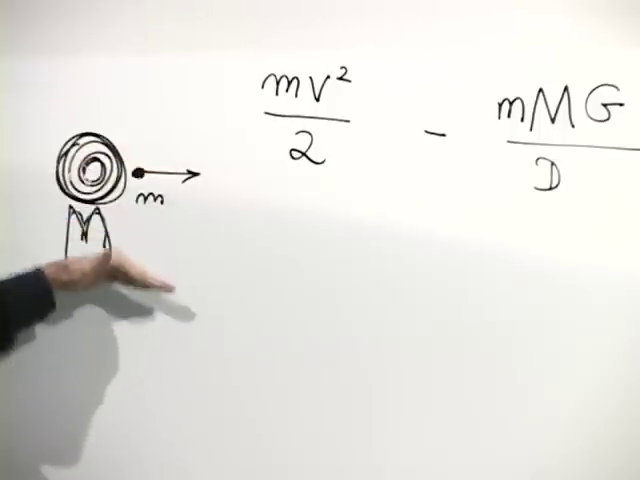
\includegraphics[width=0.62\textwidth]{lecture_02_figure_04.png}
\caption{Gesamte Newtonsche Energie einer radial bewegten Testmasse: kinetischer Term minus Gravitationspotenzial.}
\end{figure}

Das Minuszeichen ist entscheidend. Die potenzielle Energie im Gravitationsfeld ist negativ, weil die Gravitation anziehend wirkt. Nähert man das Teilchen an, nimmt die negative potenzielle Energie dem Betrag nach zu. Entfernt es sich, wird die potenzielle Energie weniger negativ.

\begin{classroomqa}
\audiencequestion{Nimmt die potenzielle Energie mit dem Abstand zu, statt abzunehmen?}\lecturetimestamp{00:34:13}
\lecturerresponse{Ja. Lassen wir die Konstanten außer Acht und betrachten die Graphen von \(1/D\) und \(-1/D\). Eine Kraft treibt das Teilchen in Richtung abnehmender potenzieller Energie. Eine anziehende Kraft entspricht daher der umgekehrten Kurve \(-1/D\): Die potenzielle Energie nimmt mit dem Abstand zu und wird negativer, wenn sich das Teilchen nach innen bewegt.}
\end{classroomqa}

\begin{figure}
\centering
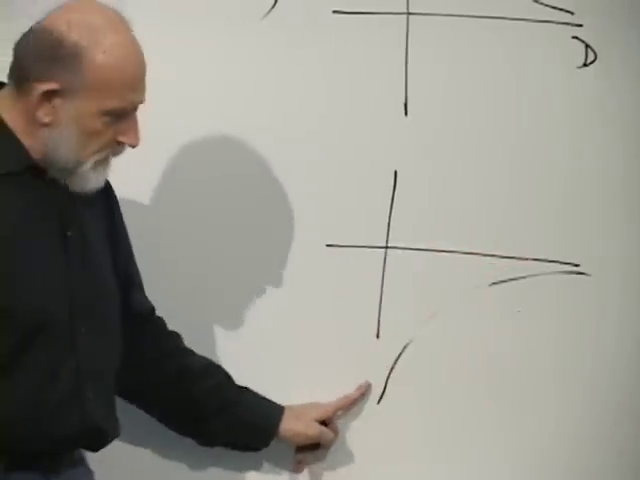
\includegraphics[width=0.46\textwidth]{lecture_02_figure_05.png}
\caption{Qualitativer Vergleich von \(1/D\) und \(-1/D\) zur Veranschaulichung des Vorzeichens der potenziellen Gravitationsenergie.}
\end{figure}

\section{Fluchtgeschwindigkeit}

Betrachten wir nun die möglichen Fälle. Die Energie kann positiv, negativ oder null sein. Andere Möglichkeiten gibt es nicht.

\begin{itemize}
\item Ist die Energie negativ, ist das Teilchen gebunden. Wirft man es mit zu geringer Geschwindigkeit nach oben, steigt es zunächst auf, wird langsamer, kehrt um und fällt zurück.
\item Ist die Energie positiv, entkommt das Teilchen. Die Gravitation bremst es zunächst ab, aber nicht genug, um es anzuhalten. Schließlich bewegt es sich mit einer asymptotisch nicht verschwindenden Geschwindigkeit nach außen.
\item Ist die Energie genau null, hat das Teilchen die Fluchtgeschwindigkeit. Das ist der Grenzfall zwischen Entkommen und Nichtentkommen.
\end{itemize}

Bei hinreichend kleiner Anfangsgeschwindigkeit dominiert von Anfang an der Potenzialterm, und die Energie ist negativ.

\begin{figure}
\centering
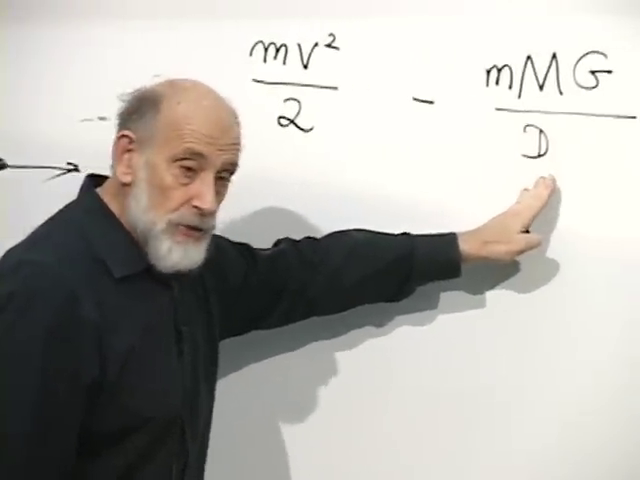
\includegraphics[width=0.62\textwidth]{lecture_02_figure_06.png}
\caption{Bei geringer Geschwindigkeit nach außen dominiert der negative Potenzialterm die Gesamtenergie.}
\end{figure}

Im Fall verschwindender Energie nimmt der Abstand weiterhin zu, während die Geschwindigkeit immer weiter abnimmt. Das Teilchen kann zu keiner endlichen Zeit zur Ruhe kommen. Denn dann würde es zurückfallen. Der Abstand ist also unbeschränkt, während die Geschwindigkeit gegen null geht.

Genau diese Analogie ist für die Kosmologie wichtig. Das Universum kann sich genauso verhalten. Ist die anfängliche Hubble-Expansion nach außen stark genug, entkommt alles allem anderen. Ist sie zu gering, setzt sich die Gravitation durch, und es kommt zu einem gewaltigen Kollaps. Dazwischen liegt der Grenzfall, der genau der Fluchtgeschwindigkeit entspricht.

\section{Newtonscher Satz}

Die kosmologische Vereinfachung beruht auf dem Newtonschen Satz für das inverse-quadratische Kraftgesetz.

Ist Materie kugelsymmetrisch um ein Zentrum verteilt, dann ist die Gravitationskraft auf ein Teilchen außerhalb der Verteilung genau dieselbe, als wäre die gesamte Masse im Zentrum konzentriert. Der Satz geht jedoch noch weiter: Befindet sich das Teilchen innerhalb der Verteilung, trägt nur die Masse innerhalb seines Radius bei. Die weiter außen liegende Masse übt insgesamt keine Kraft aus.

Die anschaulichste Fassung des Satzes betrifft eine dünne Kugelschale. Eine ideale Kugelschale übt auf ein Teilchen an jeder Stelle im Inneren keine Gravitationskraft aus, auch nicht abseits des Zentrums. Das mag zunächst überraschend sein, gilt aber für das Kraftgesetz \(1/r^2\).

\begin{classroomqa}
\audiencequestion{Bei dem Beispiel, das Sie gerade gegeben haben: Sollte es uns nicht ein wenig überraschen, dass die Kraft beim Überqueren der Grenze durch das Teilchen offenbar unstetig ist?}\lecturetimestamp{00:48:19}
\lecturerresponse{Ja. Bei einer idealen, unendlich dünnen Schale ist das überraschend und eine Besonderheit des Kraftgesetzes \(1/r^2\). Eine reale Schale hat eine Dicke, wodurch sich die Änderung glättet. Die scharfe Aussage für eine ideale Schale ist jedoch genau die bemerkenswerte Eigenschaft des Newtonschen Satzes.}
\end{classroomqa}

Eine anschauliche Analogie macht den Satz plausibel. Ersetzen wir eine Punktmasse durch eine punktförmige Wasserquelle. In drei Dimensionen nimmt die nach außen gerichtete Strömung wie \(1/r^2\) ab. Ordnet man solche Quellen lückenlos rings um eine Kugelschale an, sieht die Strömung außerhalb der Schale genauso aus, als wäre alles im Zentrum konzentriert. Innerhalb der Schale kann es keine Nettoströmung geben, denn im Zentrum befindet sich keine Quelle. Dieselbe Struktur liegt dem Gravitationssatz zugrunde.

Es geht hier nicht darum, den Satz erneut herzuleiten, sondern ihn anzuwenden.

\section{Ein homogenes Universum als Zweikörperproblem}

Kehren wir nun zur Kosmologie zurück. Betrachten wir einen kleinen Bereich des Universums, der von einem gleichmäßig verteilten Galaxiengas erfüllt ist. Man kann sich, wenn man möchte, ins Zentrum setzen. Das dient lediglich der Bequemlichkeit. Jeder kann sich selbst ins Zentrum setzen, und es muss dieselbe Gleichung herauskommen.

Wählen wir eine Galaxie auf der \(x\)-Achse mit der mitbewegten Koordinate \(x\). Da das Universum isotrop ist, spielt die Wahl der Achse keine Rolle. Zeichnen wir eine Kugel mit Mittelpunkt \(x=0\), die durch diese Galaxie verläuft. Nach Newtons Satz ist die Kraft auf die Galaxie genau dieselbe, als wäre die gesamte Masse innerhalb dieser Kugel im Zentrum konzentriert; alles außerhalb trägt nichts bei.

Die Kugel dehnt sich mit den Galaxien aus. Sie enthält stets dieselben Galaxien und damit dieselbe Gesamtmasse, obwohl sich ihr physikalischer Radius mit der Zeit verändert.

Die Bewegung dieser Galaxie erfüllt daher genau dieselbe Art von Energiegleichung wie das Projektil:
\begin{equation}
\frac{1}{2}mv^2-\frac{mMG}{D}=\text{constant}.
\end{equation}
Hier steht \(M\) nun für die Masse innerhalb der expandierenden Kugel, nicht für die zentrale Masse im einführenden Beispiel. Die Algebra vereinfacht sich, wenn man mit \(2\) multipliziert und durch \(m\) dividiert. Da eine Konstante dividiert durch \(m\) weiterhin eine Konstante ist, kann man schreiben:
\begin{equation}
v^2-\frac{2MG}{D}=\text{constant}.
\end{equation}
Auch hier bedeutet ``konstant'', dass die Größe für die betreffende Galaxie zeitlich konstant ist.

Nun setzen wir dies mit dem Skalenfaktor in Beziehung. Der physikalische Abstand zur Galaxie beträgt
\begin{equation}
D=ax,
\end{equation}
da \(x\) eine feste mitbewegte Koordinate ist. Ihre Geschwindigkeit ist
\begin{equation}
v=\dot D=\dot a\,x.
\end{equation}

Die Masse innerhalb der Kugel ist das Produkt aus Dichte und Volumen. Ist \(\rho\) die Massendichte, dann gilt
\begin{equation}
M=\frac{4\pi}{3}\rho D^3=\frac{4\pi}{3}\rho a^3x^3.
\end{equation}
Einsetzen in die Energiegleichung ergibt
\begin{equation}
\dot a^2x^2-\frac{2G}{ax}\left(\frac{4\pi}{3}\rho a^3x^3\right)=\text{constant},
\end{equation}
oder
\begin{equation}
\dot a^2x^2-\frac{8\pi G}{3}\rho a^2x^2=\text{constant}.
\end{equation}

Beide Terme auf der linken Seite sind proportional zu \(x^2\). Alles Übrige ist dort überall gleich. Daher muss auch die rechte Seite proportional zu \(x^2\) sein. Das widerspricht nicht der Bezeichnung als Konstante. Gemeint ist, dass die Größe bei festem \(x\) zeitlich konstant ist, aber von einer Galaxie zur anderen mit \(x^2\) skalieren kann. Das ist plausibel: Entferntere Galaxien bewegen sich schneller.

Kürzen wir also den gemeinsamen Faktor \(x^2\) heraus. Die verbleibende Konstante ist nun unabhängig von Zeit und Raum. Schreiben wir sie in der historisch üblichen Form als \(-k\):
\begin{equation}
\dot a^2-\frac{8\pi G}{3}\rho a^2=-k.
\end{equation}
Nach Division durch \(a^2\) gilt
\begin{equation}
\left(\frac{\dot a}{a}\right)^2=\frac{8\pi G}{3}\rho-\frac{k}{a^2}.
\end{equation}

Dies ist die berühmte Friedmann-Robertson-Walker-Gleichung, obwohl in der Vorlesung auch angemerkt wird, dass es eigentlich Friedmans Gleichung ist. Die Vorzeichenkonvention ist historisch bedingt. \(-k\) zu schreiben bedeutet nicht, dass \(k\) positiv sein muss. \(k\) kann positiv, negativ oder null sein. In Einheiten, in denen die Lichtgeschwindigkeit gleich \(1\) gesetzt wird, ist \(k\) dimensionslos.

\section{Dichte und die Gleichung für ein materiedominiertes Universum}

Die nächste Frage liegt auf der Hand: Was ist \(\rho\)? Sie ist nicht konstant. Mit der Expansion des Universums nimmt die Dichte ab.

Um diese Abhängigkeit auszudrücken, betrachten wir einen Einheitswürfel im Koordinatenraum: Er hat in \(x\), \(y\) und \(z\) jeweils eine Einheit Kantenlänge. Für alle Zeiten bleiben dieselben Galaxien in diesem Würfel, weil er sich mit den Koordinaten ausdehnt. Die Masse innerhalb dieses Koordinatenwürfels bleibt daher konstant.

\editorialnote{In der Vorlesung wird dasselbe Symbol \(M\) in mehreren Zusammenhängen verwendet. Hier steht \(M_{\Box}\) ausschließlich für die Masse in einem Koordinatenwürfel mit Einheitsvolumen, damit sie von der zuvor betrachteten zentralen Masse und der innerhalb der Kugel eingeschlossenen Masse unterschieden werden kann.}

Die physikalische Kantenlänge des Würfels ist \(a\), sein physikalisches Volumen also \(a^3\). Daher gilt
\begin{equation}
\rho=\frac{M_{\Box}}{a^3}.
\end{equation}
Dies ist der materiedominierte Fall: Auf der rechten Seite steht nur die Dichte gewöhnlicher, nichtrelativistischer Materie.

\begin{classroomqa}
\audiencequestion{Dieser Gleichung zufolge ist die Hubble-Konstante eine Funktion von \(\rho\). Sie ist also keine Konstante.}\lecturetimestamp{01:19:21}
\lecturerresponse{Genau. Die Hubble-Konstante ist nicht konstant. Sie hängt von der Dichte ab, und die Dichte verändert sich mit der Zeit. In der Vorlesung wird sogar scherzhaft vorgeschlagen, die Abschlussprüfung könnte aus einer einzigen Frage bestehen: Ist die Hubble-Konstante konstant?}
\end{classroomqa}

Setzt man \(\rho=M_{\Box}/a^3\) in die Friedmann-Gleichung ein, erhält man
\begin{equation}
\left(\frac{\dot a}{a}\right)^2=\frac{8\pi G M_{\Box}}{3a^3}-\frac{k}{a^2}.
\end{equation}

Damit sind die willkürlichen Festlegungen klar: Man benötigt die Masse in einem Koordinatenwürfel mit Einheitsvolumen und den Wert von \(k\). Die drei möglichen Vorzeichen von \(k\) entsprechen den drei Energiefällen des Projektilproblems.

\begin{itemize}
\item Wenn \(-k>0\), liegt die Energie gewissermaßen über der Fluchtgeschwindigkeit, und das Universum dehnt sich ewig aus.
\item Wenn \(-k<0\), setzt sich die Gravitation schließlich durch, und das Universum kollabiert wieder.
\item Wenn \(k=0\), entspricht das Universum genau der Fluchtgeschwindigkeit.
\end{itemize}

\begin{classroomqa}
\audiencequestion{Ist \(k=0\)? Nähert sich dann die Geschwindigkeit zwischen zwei Galaxien null?}\lecturetimestamp{01:21:12}
\lecturerresponse{Ja. Im kritischen Fall geht die Geschwindigkeit gegen null, der Abstand bleibt jedoch unbeschränkt. Die Galaxien entfernen sich weiterhin voneinander, aber immer langsamer. Kämen sie zu irgendeinem endlichen Zeitpunkt tatsächlich zum Stillstand, würden sie zurückfallen.}
\end{classroomqa}

\section{Der kritische Fall \(k=0\)}

Betrachten wir nun den einfachsten Fall, \(k=0\). Das ist genau der Fall der Fluchtgeschwindigkeit. Er ist nur deshalb einfacher, weil die Mathematik einfacher ist. Die Gleichung lautet
\begin{equation}
\left(\frac{\dot a}{a}\right)^2=\frac{8\pi G M_{\Box}}{3a^3}.
\end{equation}

Die rechte Seite ist stets positiv und niemals null. Daher kann \(\dot a/a\) nicht null werden. In diesem Fall kann das Universum nicht umkehren. Es dehnt sich entweder ständig aus oder zieht sich ständig zusammen. Betrachten wir den expandierenden Zweig.

Nehmen wir nun ein Potenzgesetz an:
\begin{equation}
a(t)=ct^p.
\end{equation}
Dann gilt
\begin{equation}
\dot a = cp\,t^{p-1},
\end{equation}
also
\begin{equation}
\frac{\dot a}{a}=\frac{p}{t}.
\end{equation}
Einsetzen in die Differentialgleichung ergibt
\begin{equation}
\frac{p^2}{t^2}=\frac{8\pi G M_{\Box}}{3c^3t^{3p}}.
\end{equation}
Damit die Potenzen von \(t\) übereinstimmen, muss gelten:
\begin{equation}
3p=2.
\end{equation}
Also
\begin{equation}
p=\frac{2}{3}.
\end{equation}
Dann müssen die Konstanten die Bedingung erfüllen
\begin{equation}
\frac{4}{9}=\frac{8\pi G M_{\Box}}{3c^3},
\end{equation}
daraus folgt
\begin{equation}
c^3=6\pi G M_{\Box}.
\end{equation}
Somit gilt
\begin{equation}
a(t)=\left(6\pi G M_{\Box}\right)^{1/3}t^{2/3}.
\end{equation}

Eine additive Verschiebung der Zeit ist weiterhin möglich. Sie wird berücksichtigt, indem man \(t\) durch \(t-t_0\) ersetzt. Wählt man den Zeitursprung so, dass \(a=0\) bei \(t=0\) gilt, entfällt diese verbleibende Konstante.

Das Universum dehnt sich also mit der Zeit hoch zwei Drittel aus:
\begin{equation}
a(t)\propto t^{2/3}.
\end{equation}
Die Expansion verläuft nicht linear mit der Zeit. Lineares Wachstum entspräche einer unbeschleunigten Bewegung. Hier verlangsamt sich die Expansion.

Extrapoliert man die Formel zurück bis \(t=0\), geht der Skalenfaktor gegen null und die Dichte wächst unbegrenzt. Die Aussage \(a=0\) ist eine extreme Idealisierung. Wir wissen nicht, was mit Materie geschieht, wenn sie zu dicht wird. Entscheidend ist, dass zu einem frühen Zeitpunkt alles so dicht gedrängt war, dass Atome, Atomkerne und Quarks in einem außergewöhnlich dichten Zustand zusammengepackt waren.

\section{Die Hubble-Konstante und das Alter des Universums}

Im kritischen Modell gilt
\begin{equation}
H(t)=\frac{\dot a}{a}=\frac{2}{3t}.
\end{equation}
Die Hubble-Konstante ist also näherungsweise der Kehrwert des Alters des Universums:
\begin{equation}
t=\frac{2}{3H}.
\end{equation}
Das ist eines der wichtigsten Ergebnisse der Rechnung. Misst man heute die Hubble-Konstante, erhält man eine Schätzung des Alters des Universums, zumindest bis zu dem Zeitpunkt zurück, an dem das Newtonsche Modell seine Gültigkeit verliert.

Das angegebene Alter beträgt ungefähr \(13\) bis \(14\) Milliarden Jahre. Im Text heißt es außerdem, dass \(k=0\) beobachtungsmäßig sehr realistisch ist: Bei der dort angegebenen Genauigkeit ist keine signifikante Abweichung von \(k=0\) bekannt.

\begin{classroomqa}
\audiencequestion{Ich bin etwas verwirrt darüber, was \(M\) und \(a\) sind.}\lecturetimestamp{01:39:16}
\lecturerresponse{Beide hängen von der willkürlichen Wahl des Koordinatengitters ab. Ändert man das Bezugsvolumen, ändert sich die darin enthaltene Materiemenge, und auch der Zahlenwert des Skalenfaktors ändert sich. Physikalisch sind die Dichte \(M/a^3\) oder äquivalent dazu Kombinationen wie \(a/M^{1/3}\), die nicht davon abhängen, wie das Koordinatengitter gewählt wurde. In der Lösung mit \(k=0\) kürzt sich die unbekannte Konstante vor \(t^{2/3}\) aus \(\dot a/a\) heraus. Deshalb hängt die Altersbeziehung \(t=2/3H\) nicht von der Masse im Bezugsvolumen ab.}
\end{classroomqa}

In der Lösung sieht man diese Kürzung unmittelbar. Ist
\begin{equation}
a(t)=Ct^{2/3},
\end{equation}
dann gilt
\begin{equation}
\dot a=\frac{2}{3}Ct^{-1/3},
\end{equation}
und damit
\begin{equation}
\frac{\dot a}{a}=\frac{2}{3t}.
\end{equation}
Die Konstante \(C\) fällt vollständig heraus.

\section{Warum die Newtonsche Herleitung funktioniert}

Gegen Ende stellt sich die Frage: Warum stimmt die Newtonsche Herleitung so gut mit der relativistischen überein?

\begin{classroomqa}
\audiencequestion{Das scheint alles von der Annahme eines offenen Universums abzuhängen.}\lecturetimestamp{01:45:44}
\lecturerresponse{Die Herleitung ist an dieser Stelle Newtonsch, und Newtonsche Physik setzt einen flachen Raum voraus. Die geometrische Deutung von \(k\) wird auf die nächste Vorlesung verschoben. Dort wird \(k=0\) einem flachen Raum entsprechen, während die anderen Vorzeichen mit einer gekrümmten räumlichen Geometrie verknüpft werden.}
\end{classroomqa}

\begin{classroomqa}
\audiencequestion{Hing die Länge von Meterstäben vor langer Zeit von \(a\) ab?}\lecturetimestamp{01:47:53}
\lecturerresponse{Weit genug zurück in der Zeit wäre die Materie so dicht gedrängt gewesen, dass es keine voneinander getrennten Meterstäbe mehr gegeben hätte. Zuvor wären sie zusammengedrückt worden. In der Vorlesung wird außerdem daran erinnert, dass die Relativitätstheorie vollkommen starre Körper ohnehin nicht zulässt: Wäre ein Körper vollkommen starr, würde ein Stoß auf der einen Seite augenblicklich ein Signal zur anderen Seite senden, also schneller als das Licht.}
\end{classroomqa}

\begin{classroomqa}
\audiencequestion{Warum glauben Sie, dass die Newtonsche und die relativistische Gleichung hier übereinstimmen?}\lecturetimestamp{01:49:03}
\lecturerresponse{Weil die Newtonsche Beschreibung nur auf einen hinreichend kleinen Bereich angewandt wird. Solange dieser Bereich klein gegenüber dem Krümmungsradius des gesamten Universums ist und die lokalen Hubble-Geschwindigkeiten darin deutlich unter der Lichtgeschwindigkeit liegen, ist die Newtonsche Mechanik eine gute Näherung. Die Vorlesung vergleicht dies mit der Untersuchung des Graswachstums auf der Erde: Man kann den lokalen Vorgang verstehen, ohne die Krümmung der gesamten Erde heranzuziehen.}
\end{classroomqa}

Das ist die Logik des lokalen Bereichs. Die Newtonsche Mechanik setzt erstens voraus, dass die Raumkrümmung für die betrachtete Frage keine wesentliche Rolle spielt, und zweitens, dass sich lokal nichts annähernd mit Lichtgeschwindigkeit bewegt. In der Kosmologie bedeutet das, einen Bereich zu wählen, der groß genug ist, um homogen zu sein, aber klein genug, dass Krümmungseffekte vernachlässigbar sind und die Hubble-Geschwindigkeiten nichtrelativistisch bleiben.

Vor diesem Hintergrund ist die Newtonsche Rechnung kein Zufall. Sie ist die lokale Näherung einer Gleichung, die sich auch relativistisch lesen lässt. Bringt man den Krümmungsterm auf die linke Seite, erhält man aus der Friedmann-Gleichung
\begin{equation}
\left(\frac{\dot a}{a}\right)^2+\frac{k}{a^2}=\frac{8\pi G}{3}\rho.
\end{equation}
Die linke Seite ist geometrischer Natur: Sie enthält den Skalenfaktor und, wie wir nächstes Mal sehen werden, die Raumkrümmung. Auf der rechten Seite steht die Energiedichte. Das ist genau die Art von Gleichung, die man von der allgemeinen Relativitätstheorie erwartet.

Nächstes Mal geht es um die Krümmung selbst, Einsteins Gleichungen und den Zusammenhang zwischen der relativistischen und der Newtonschen Herleitung.
